%%%%%%%%%%%%%%%%%%%%%%%%%%%%%%%%%%%%%%%%%%%%%%%%%%%%%%%%%%%%%%%%%%%%%%%%%%%%%%
%
% Appendix file included in main project file using \input{}
%
% Assumes that LaTeX2e macros and packages defined in cg_comp.sty are
%   available
%
%%%%%%%%%%%%%%%%%%%%%%%%%%%%%%%%%%%%%%%%%%%%%%%%%%%%%%%%%%%%%%%%%%%%%%%%%%%%%%

 \newpage
 \section{Other Classical Guitar String Sets\label{app:specs}}

 \subsection{Light Tension}

 \begin{table}[htbp]
  \centering
  \caption{\label{tbl:ej43_ips} String properties for the D'Addario Pro-Arte Nylon Classical Guitar Strings -- Light Tension (EJ43). The corresponding scale length is 25.5~inches.}
    \begin{tabular}{lcccc}
    \hline \hline
    String  & Note  & \multicolumn{1}{l}{Diameter (in)} & \multicolumn{1}{l}{Density (lb/in)} & \multicolumn{1}{l}{Tension (lb)} \\
    \hline
    J4301 & E$_4$  & 0.0275 & $2.024 \times 10^{-5}$ & 14.8 \\
    J4302 & B$_3$  & 0.0317 & $2.729 \times 10^{-5}$ & 11.2 \\
    J4303 & G$_3$  & 0.0397 & $4.525 \times 10^{-5}$ & 11.7 \\
    J4304 & D$_3$  & 0.0280 & $1.020 \times 10^{-4}$ & 14.8 \\
    J4305 & A$_2$  & 0.0330 & $1.535 \times 10^{-4}$ & 12.5 \\
    J4306 & E$_2$  & 0.0420 & $2.888 \times 10^{-4}$ & 13.2 \\
    \hline
    \end{tabular}%
 \end{table}%

 \begin{table}[htbp]
  \centering
  \caption{\label{tbl:ej43_mks} String properties for the D'Addario Pro-Arte Nylon Classical Guitar Strings -- Light Tension (EJ43). The corresponding scale length is 650~mm.}
    \begin{tabular}{lcccc}
    \hline \hline
    String  & Note  & \multicolumn{1}{l}{Radius (mm)} & \multicolumn{1}{l}{Density (kg/mm)} & \multicolumn{1}{l}{Tension (N)} \\
    \hline
    J4301 & E$_4$  & 0.349 & $3.615 \times 10^{-7}$ & 66.4 \\
    J4302 & B$_3$  & 0.403 & $4.875 \times 10^{-7}$ & 50.2 \\
    J4303 & G$_3$  & 0.504 & $8.083 \times 10^{-7}$ & 52.5 \\
    J4304 & D$_3$  & 0.356 & $1.823 \times 10^{-6}$ & 66.4 \\
    J4305 & A$_2$  & 0.419 & $2.741 \times 10^{-6}$ & 56.1 \\
    J4306 & E$_2$  & 0.533 & $5.159 \times 10^{-6}$ & 59.2 \\
    \hline
    \end{tabular}%
 \end{table}%

 \begin{table}[htbp]
  \centering
  \caption{\label{tbl:ej43_props} Derived physical properties of the D'Addario Pro-Arte Nylon Classical Guitar Strings -- Light Tension (EJ43). The corresponding scale length is 650 mm.}
    \begin{tabular}{lcccc}
    \hline \hline
    String  & $R$ & $\kappa$ & Modulus (GPa) & Stiffness \\
    \hline
    J4301 & 2.67 $\times 10^{4}$ & 29.8 & 5.17 & 2.94 $\times 10^{-3}$ \\
    J4302 & 1.09 $\times 10^{4}$ & 11.6 & 1.14 & 2.11 $\times 10^{-3}$ \\
    J4303 & 6.63 $\times 10^{4}$ & 75.6 & 4.97 & 6.75 $\times 10^{-3}$ \\
    J4304 & 2.60 $\times 10^{4}$ & 29.1 & 4.86 & 2.95 $\times 10^{-3}$ \\
    J4305 & 2.66 $\times 10^{4}$ & 29.7 & 3.02 & 3.52 $\times 10^{-3}$ \\
    J4306 & 1.40 $\times 10^{4}$ & 15.2 & 1.01 & 3.20 $\times 10^{-3}$ \\
    \hline
    \end{tabular}%
 \end{table}%

 \begin{table}[htbp]
  \centering
  \caption{\label{tbl:ej43_setbacks} Predicted setbacks for the D'Addario Pro-Arte Nylon Classical Guitar Strings -- Light Tension (EJ43) on the Alhambra 8P classical guitar.}
    \begin{tabular}{lcccc}
    \hline \hline
    String  & $\Delta S$~(mm) & $\Delta N$~(mm) \\
    \hline
    J4301 & 1.91 & -0.31 \\
    J4302 & 1.37 & -0.12 \\
    J4303 & 4.38 & -0.79 \\
    J4304 & 1.92 & -0.30 \\
    J4305 & 2.29 & -0.31 \\
    J4306 & 2.08 & -0.16 \\
    \hline \hline
    Mean & 2.32 & -0.33 \\
    \hline
    \end{tabular}%
 \end{table}%

 \begin{figure}
  \centering
  \begin{subfigure}[b]{0.45\textwidth}
   \centering
   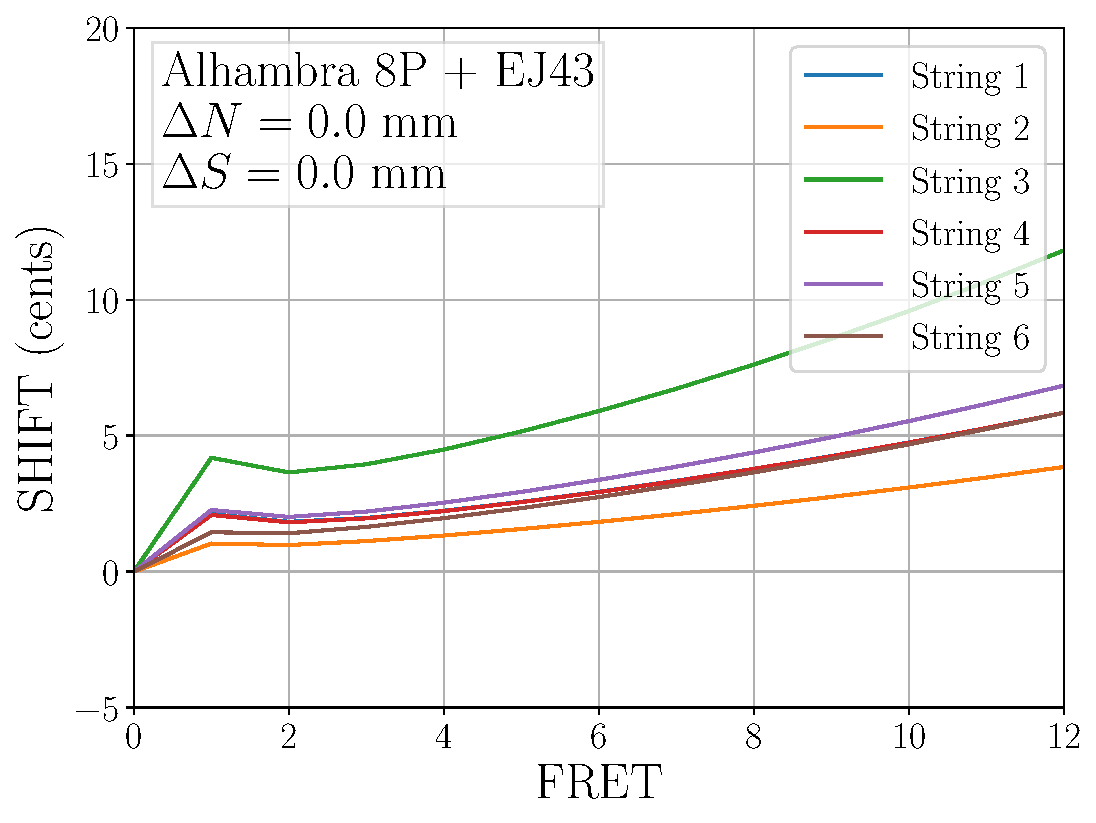
\includegraphics[width=3.25in]{figures/shift_alhambra8p_ej43_null}
   \caption{Uncompensated}
   \label{fig:shift_alhambra8p_ej43_null}
  \end{subfigure}
  \hspace{0.25in}
  \begin{subfigure}[b]{0.45\textwidth}
   \centering
   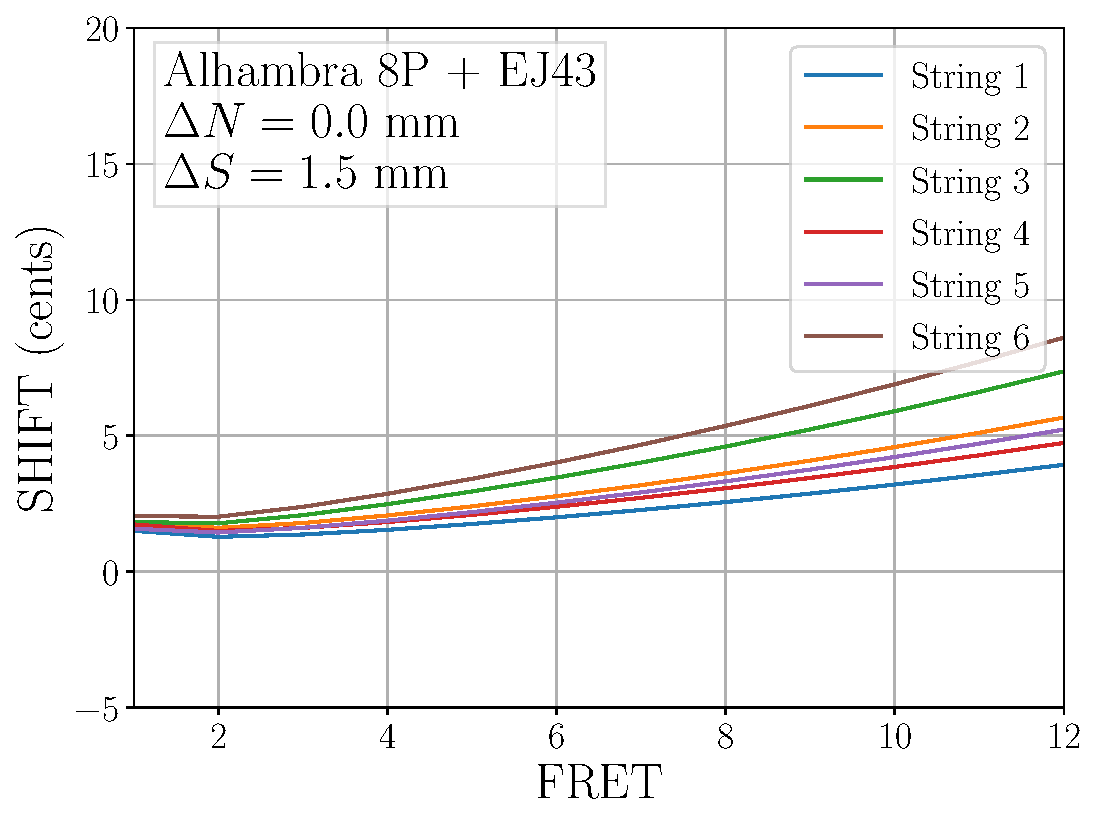
\includegraphics[width=3.25in]{figures/shift_alhambra8p_ej43_factory}
   \caption{Factory guitar}
   \label{fig:shift_alhambra8p_ej43_factory}
  \end{subfigure}
  \par\vspace{0.25in}
  \begin{subfigure}[b]{0.45\textwidth}
   \centering
   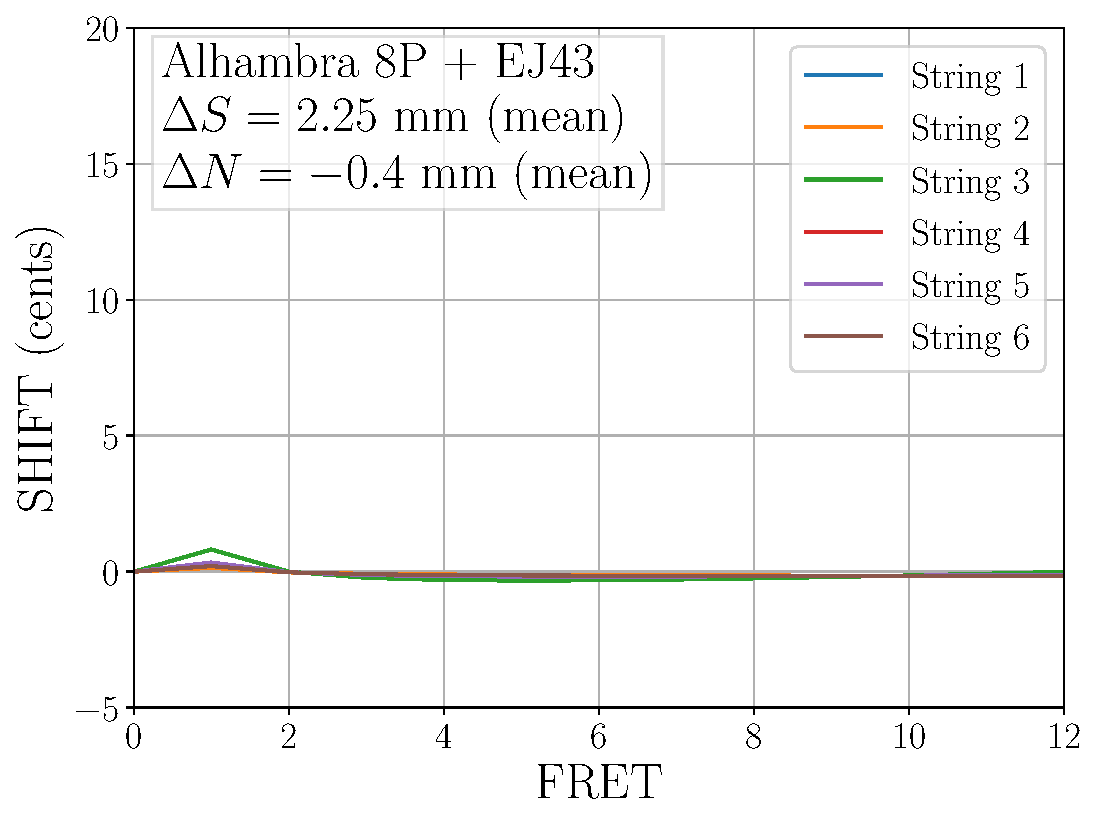
\includegraphics[width=3.25in]{figures/shift_alhambra8p_ej43_full}
   \caption{Full compensation}
   \label{fig:shift_alhambra8p_ej43_full}
  \end{subfigure}
  \hspace{0.25in}
  \begin{subfigure}[b]{0.45\textwidth}
   \centering
   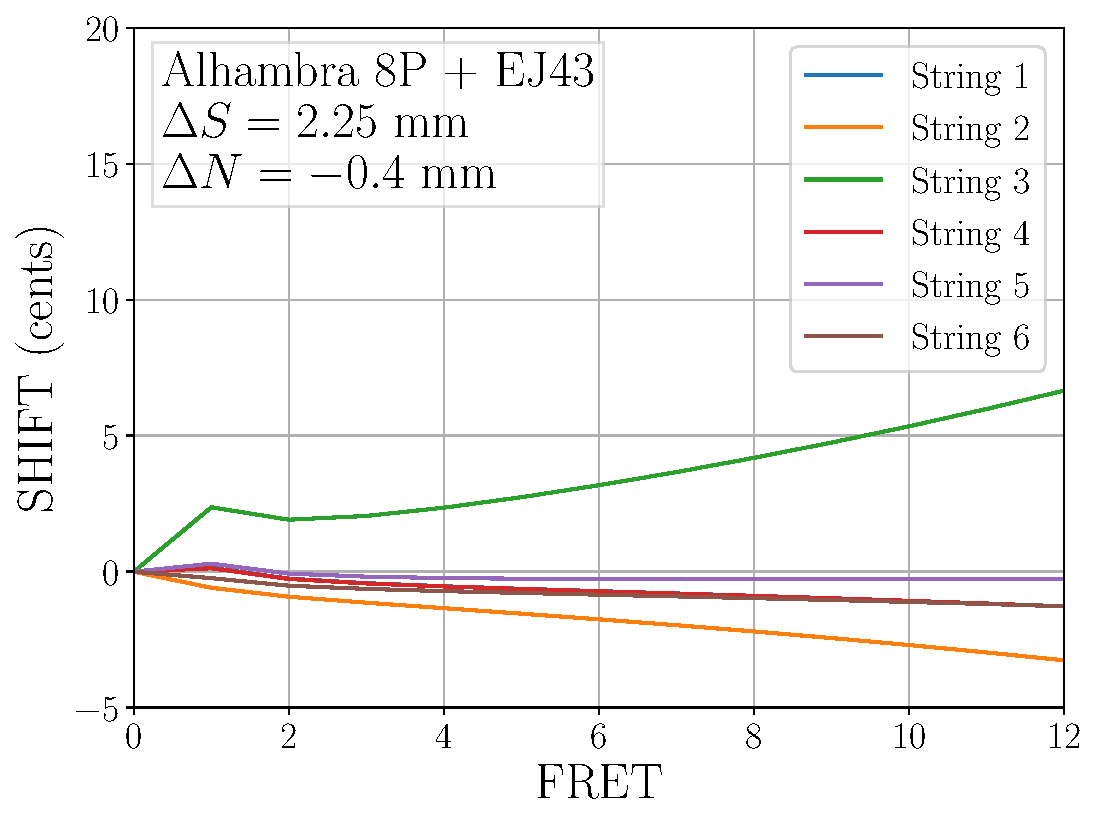
\includegraphics[width=3.25in]{figures/shift_alhambra8p_ej43_mean}
   \caption{Mean compensation}
   \label{fig:shift_alhambra8p_ej43_mean}
  \end{subfigure}
  \caption{\label{fig:compensation_alhambra8p_ej43} Frequency shift (in cents) for an Alhambra 8P guitar with D'Addario Pro-Arte Nylon Classical Guitar Strings -- Light Tension (EJ43). Four different strategies of saddle and nut compensation are illustrated.}
 \end{figure}

 \newpage
 \subsection{Hard Tension}

 \begin{table}[htbp]
  \centering
  \caption{\label{tbl:ej46_ips} String properties for the D'Addario Pro-Arte Nylon Classical Guitar Strings -- Hard Tension (EJ46). The corresponding scale length is 25.5~inches.}
    \begin{tabular}{lcccc}
    \hline \hline
    String  & Note  & \multicolumn{1}{l}{Diameter (in)} & \multicolumn{1}{l}{Density (lb/in)} & \multicolumn{1}{l}{Tension (lb)} \\
    \hline
    J4601 & E$_4$  & 0.0285 & $2.161 \times 10^{-5}$ & 15.8 \\
    J4602 & B$_3$  & 0.0327 & $2.924 \times 10^{-5}$ & 12.0 \\
    J4603 & G$_3$  & 0.0410 & $4.795 \times 10^{-5}$ & 12.4 \\
    J4604 & D$_3$  & 0.0300 & $1.124 \times 10^{-4}$ & 16.3 \\
    J4605 & A$_2$  & 0.0360 & $1.952 \times 10^{-4}$ & 15.9 \\
    J4606 & E$_2$  & 0.0440 & $3.173 \times 10^{-4}$ & 14.5 \\
    \hline
    \end{tabular}%
 \end{table}%

 \begin{table}[htbp]
  \centering
  \caption{\label{tbl:ej46_mks} String properties for the D'Addario Pro-Arte Nylon Classical Guitar Strings -- Hard Tension (EJ46). The corresponding scale length is 650~mm.}
    \begin{tabular}{lcccc}
    \hline \hline
    String  & Note  & \multicolumn{1}{l}{Radius (mm)} & \multicolumn{1}{l}{Density (kg/mm)} & \multicolumn{1}{l}{Tension (N)} \\
    \hline
    J4601 & E$_4$  & 0.362 & $3.860 \times 10^{-7}$ & 70.9 \\
    J4602 & B$_3$  & 0.415 & $5.223 \times 10^{-7}$ & 53.8 \\
    J4603 & G$_3$  & 0.521 & $8.565 \times 10^{-7}$ & 55.6 \\
    J4604 & D$_3$  & 0.381 & $2.007 \times 10^{-6}$ & 73.1 \\
    J4605 & A$_2$  & 0.457 & $3.487 \times 10^{-6}$ & 71.3 \\
    J4606 & E$_2$  & 0.559 & $5.667 \times 10^{-6}$ & 65.0 \\
    \hline
    \end{tabular}%
 \end{table}%

 \begin{table}[htbp]
  \centering
  \caption{\label{tbl:ej46_props} Derived physical properties of the D'Addario Pro-Arte Nylon Classical Guitar Strings -- Hard Tension (EJ46). The corresponding scale length is 650 mm.}
    \begin{tabular}{lcccc}
    \hline \hline
    String  & $R$ & $\kappa$ & Modulus (GPa) & Stiffness \\
    \hline
    J4601 & 10.2 $\times 10^{4}$ & 116.5 & 20.1 & 6.01 $\times 10^{-3}$ \\
    J4602 & 4.13 $\times 10^{4}$ & 46.7 & 4.65 & 4.37 $\times 10^{-3}$ \\
    J4603 & 2.96 $\times 10^{4}$ & 33.2 & 2.16 & 4.61 $\times 10^{-3}$ \\
    J4604 & 4.66 $\times 10^{4}$ & 52.8 & 8.47 & 4.26 $\times 10^{-3}$ \\
    J4605 & 1.79 $\times 10^{4}$ & 19.7 & 2.13 & 3.12 $\times 10^{-3}$ \\
    J4606 & 2.65 $\times 10^{4}$ & 29.6 & 1.96 & 4.68 $\times 10^{-3}$ \\
    \hline
    \end{tabular}%
 \end{table}%

 \begin{table}[htbp]
  \centering
  \caption{\label{tbl:ej46_setbacks} Predicted setbacks for the D'Addario Pro-Arte Nylon Classical Guitar Strings -- Hard Tension (EJ46) on the Alhambra 8P classical guitar.}
    \begin{tabular}{lcccc}
    \hline \hline
    String  & $\Delta S$~(mm) & $\Delta N$~(mm) \\
    \hline
    J4601 & 3.91 & -1.20 \\
    J4602 & 2.84 & -0.49 \\
    J4603 & 3.00 & -0.34 \\
    J4604 & 2.77 & -0.55 \\
    J4605 & 2.03 & -0.20 \\
    J4606 & 3.04 & -0.31 \\
    \hline \hline
    Mean & 2.93 & -0.52 \\
    \hline
    \end{tabular}%
 \end{table}%

 \begin{figure}
  \centering
  \begin{subfigure}[b]{0.45\textwidth}
   \centering
   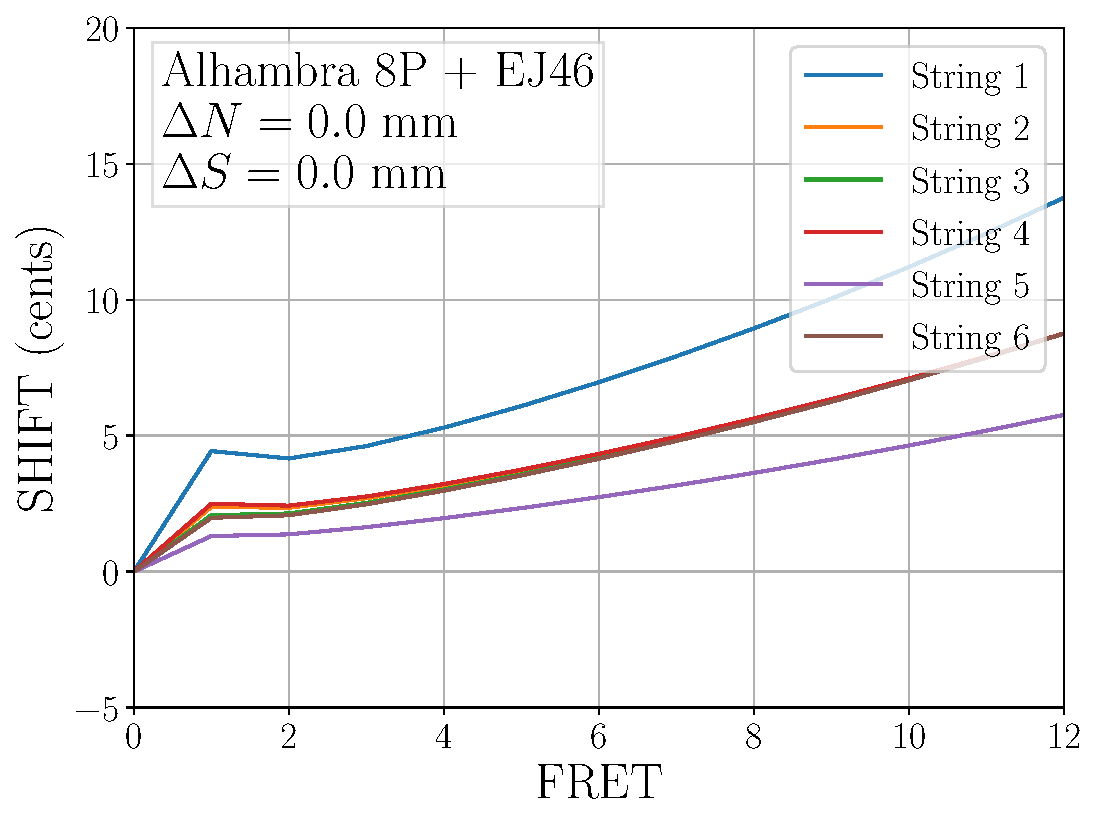
\includegraphics[width=3.25in]{figures/shift_alhambra8p_ej46_null}
   \caption{Uncompensated}
   \label{fig:shift_alhambra8p_ej46_null}
  \end{subfigure}
  \hspace{0.25in}
  \begin{subfigure}[b]{0.45\textwidth}
   \centering
   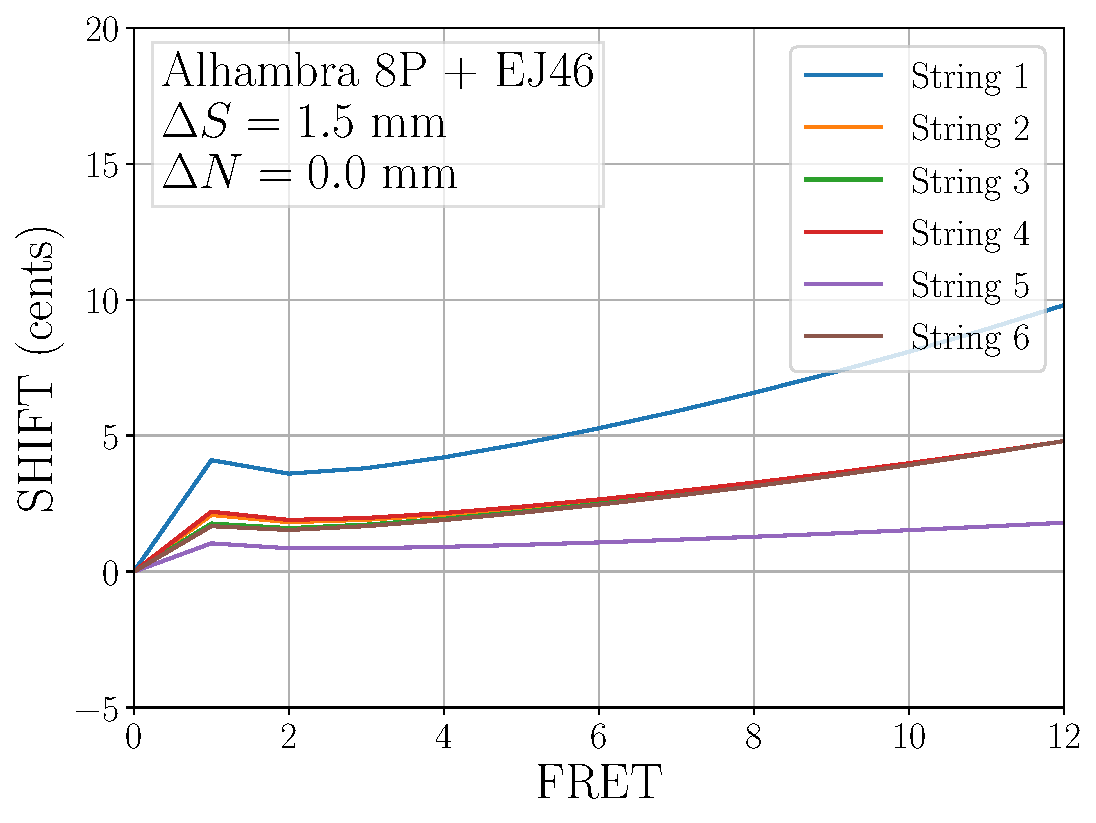
\includegraphics[width=3.25in]{figures/shift_alhambra8p_ej46_factory}
   \caption{Factory guitar}
   \label{fig:shift_alhambra8p_ej46_factory}
  \end{subfigure}
  \par\vspace{0.25in}
  \begin{subfigure}[b]{0.45\textwidth}
   \centering
   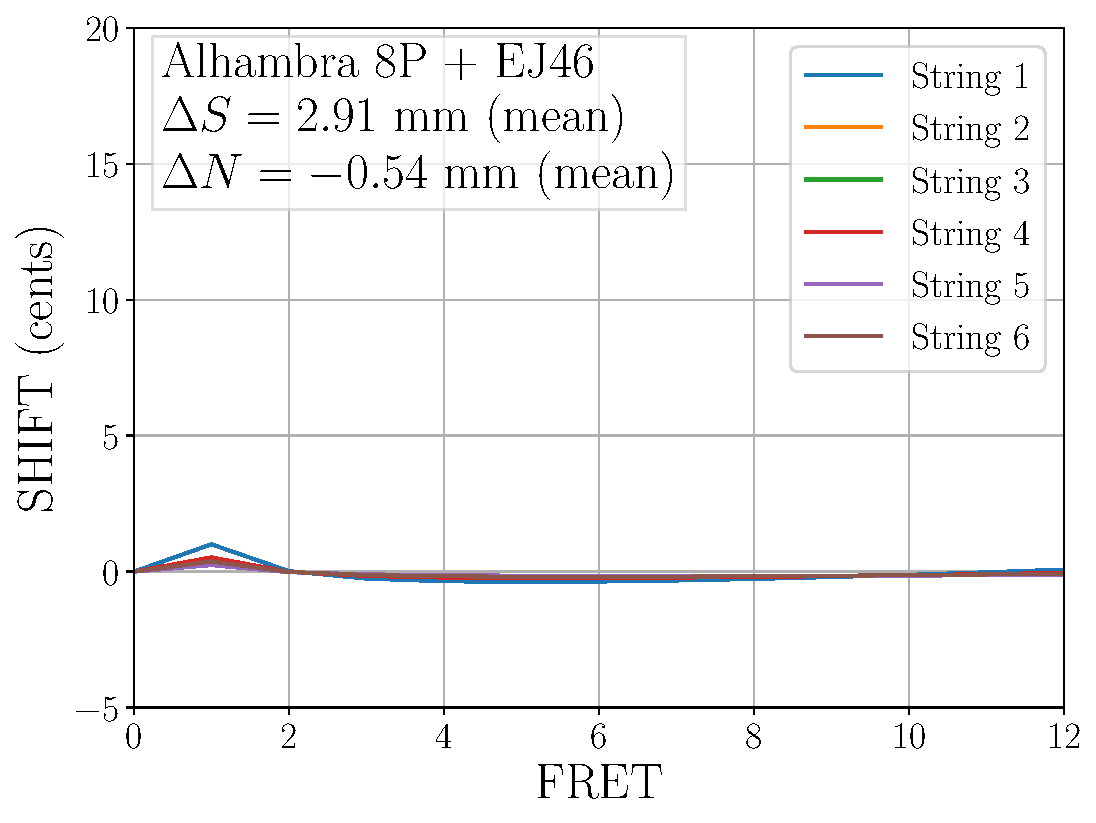
\includegraphics[width=3.25in]{figures/shift_alhambra8p_ej46_full}
   \caption{Full compensation}
   \label{fig:shift_alhambra8p_ej46_full}
  \end{subfigure}
  \hspace{0.25in}
  \begin{subfigure}[b]{0.45\textwidth}
   \centering
   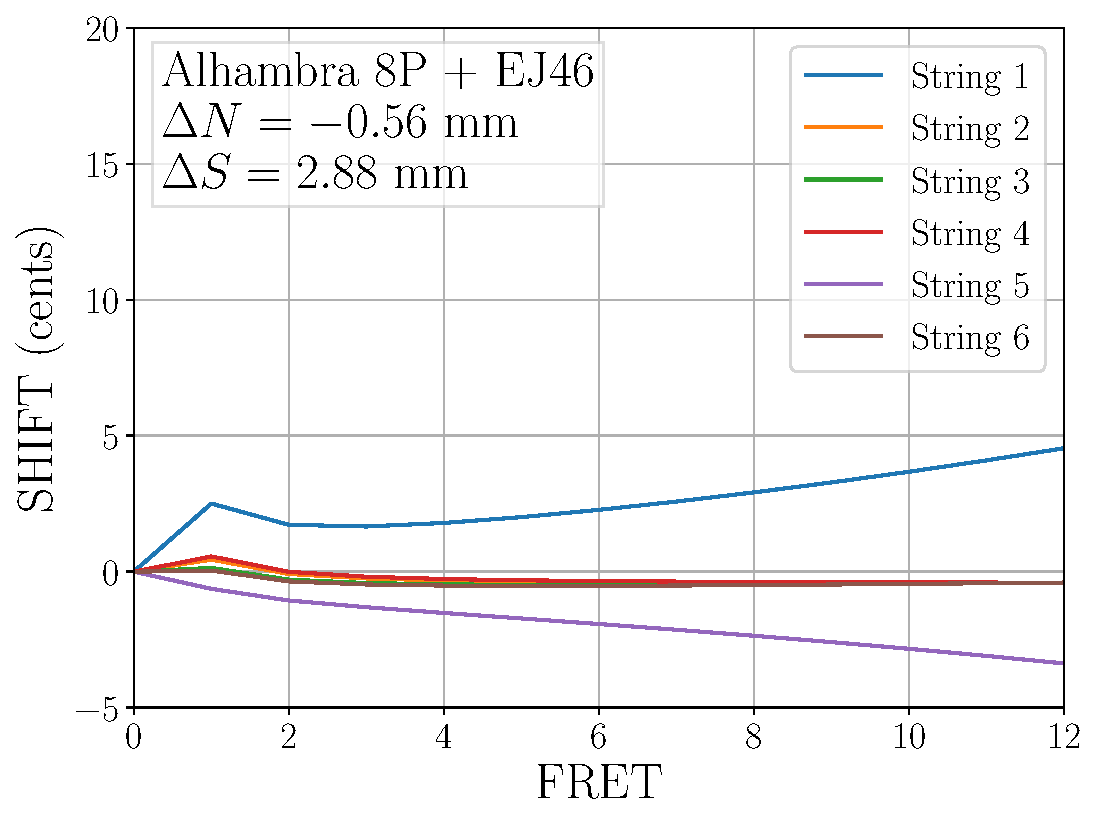
\includegraphics[width=3.25in]{figures/shift_alhambra8p_ej46_mean}
   \caption{Mean compensation}
   \label{fig:shift_alhambra8p_ej46_mean}
  \end{subfigure}
  \caption{\label{fig:compensation_alhambra8p_ej46} Frequency shift (in cents) for an Alhambra 8P guitar with D'Addario Pro-Arte Nylon Classical Guitar Strings -- Hard Tension (EJ46). Four different strategies of saddle and nut compensation are illustrated.}
 \end{figure}

 \newpage
 \subsection{Extra Hard Tension}

 \begin{table}[htbp]
  \centering
  \caption{\label{tbl:ej44_ips} String properties for the D'Addario Pro-Arte Nylon Classical Guitar Strings -- Extra Hard Tension (EJ44). The corresponding scale length is 25.5~inches.}
    \begin{tabular}{lcccc}
    \hline \hline
    String  & Note  & \multicolumn{1}{l}{Diameter (in)} & \multicolumn{1}{l}{Density (lb/in)} & \multicolumn{1}{l}{Tension (lb)} \\
    \hline
    J4401 & E$_4$  & 0.0290 & $2.243 \times 10^{-5}$ & 16.4 \\
    J4402 & B$_3$  & 0.0333 & $3.046 \times 10^{-5}$ & 12.5 \\
    J4403 & G$_3$  & 0.0416 & $4.989 \times 10^{-5}$ & 12.9 \\
    J4404 & D$_3$  & 0.0300 & $1.124 \times 10^{-4}$ & 16.3 \\
    J4405 & A$_2$  & 0.0360 & $1.952 \times 10^{-4}$ & 15.9 \\
    J4406 & E$_2$  & 0.0450 & $3.435 \times 10^{-4}$ & 15.7 \\
    \hline
    \end{tabular}%
 \end{table}%

 \begin{table}[htbp]
  \centering
  \caption{\label{tbl:ej44_mks} String properties for the D'Addario Pro-Arte Nylon Classical Guitar Strings -- Extra Hard Tension (EJ44). The corresponding scale length is 650~mm.}
    \begin{tabular}{lcccc}
    \hline \hline
    String  & Note  & \multicolumn{1}{l}{Radius (mm)} & \multicolumn{1}{l}{Density (kg/mm)} & \multicolumn{1}{l}{Tension (N)} \\
    \hline
    J4401 & E$_4$  & 0.368 & $4.007 \times 10^{-7}$ & 73.6 \\
    J4402 & B$_3$  & 0.423 & $5.441 \times 10^{-7}$ & 56.1 \\
    J4403 & G$_3$  & 0.528 & $8.912 \times 10^{-7}$ & 57.9 \\
    J4404 & D$_3$  & 0.381 & $2.007 \times 10^{-6}$ & 73.1 \\
    J4405 & A$_2$  & 0.457 & $3.487 \times 10^{-6}$ & 71.3 \\
    J4406 & E$_2$  & 0.571 & $6.136 \times 10^{-6}$ & 70.4 \\
    \hline
    \end{tabular}%
 \end{table}%

 \begin{table}[htbp]
  \centering
  \caption{\label{tbl:ej44_props} Derived physical properties of the D'Addario Pro-Arte Nylon Classical Guitar Strings -- Extra Hard Tension (EJ44). The corresponding scale length is 650 mm.}
    \begin{tabular}{lcccc}
    \hline \hline
    String  & $R$ & $\kappa$ & Modulus (GPa) & Stiffness \\
    \hline
    J4401 & 2.47 $\times 10^{4}$ & 27.6 & 20.1 & 2.98 $\times 10^{-3}$ \\
    J4402 & 5.64 $\times 10^{4}$ & 64.2 & 4.65 & 5.21 $\times 10^{-3}$ \\
    J4403 & 6.21 $\times 10^{4}$ & 70.7 & 2.16 & 6.83 $\times 10^{-3}$ \\
    J4404 & 4.66 $\times 10^{4}$ & 52.8 & 8.47 & 4.26 $\times 10^{-3}$ \\
    J4405 & 1.79 $\times 10^{4}$ & 19.7 & 2.13 & 3.12 $\times 10^{-3}$ \\
    J4406 & 2.56 $\times 10^{4}$ & 28.5 & 1.96 & 4.70 $\times 10^{-3}$ \\
    \hline
    \end{tabular}%
 \end{table}%

 \begin{table}[htbp]
  \centering
  \caption{\label{tbl:ej44_setbacks} Predicted setbacks for the D'Addario Pro-Arte Nylon Classical Guitar Strings -- Extra Hard Tension (EJ44) on the Alhambra 8P classical guitar.}
    \begin{tabular}{lcccc}
    \hline \hline
    String  & $\Delta S$~(mm) & $\Delta N$~(mm) \\
    \hline
    J4401 & 1.93 & -0.29 \\
    J4402 & 3.39 & -0.67 \\
    J4403 & 4.44 & -0.73 \\
    J4404 & 2.77 & -0.55 \\
    J4405 & 2.03 & -0.20 \\
    J4406 & 3.05 & -0.30 \\
    \hline \hline
    Mean & 2.94 & -0.46 \\
    \hline
    \end{tabular}%
 \end{table}%

 \begin{figure}
  \centering
  \begin{subfigure}[b]{0.45\textwidth}
   \centering
   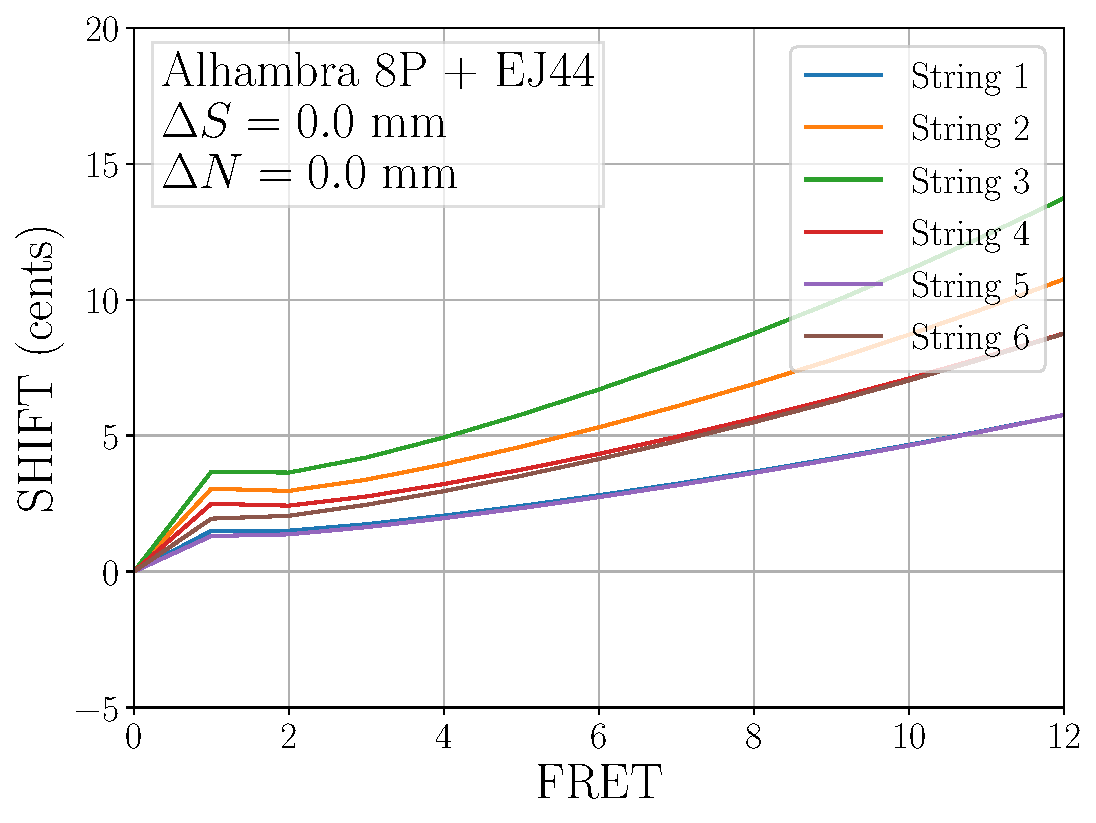
\includegraphics[width=3.25in]{figures/shift_alhambra8p_ej44_null}
   \caption{Uncompensated}
   \label{fig:shift_alhambra8p_ej44_null}
  \end{subfigure}
  \hspace{0.25in}
  \begin{subfigure}[b]{0.45\textwidth}
   \centering
   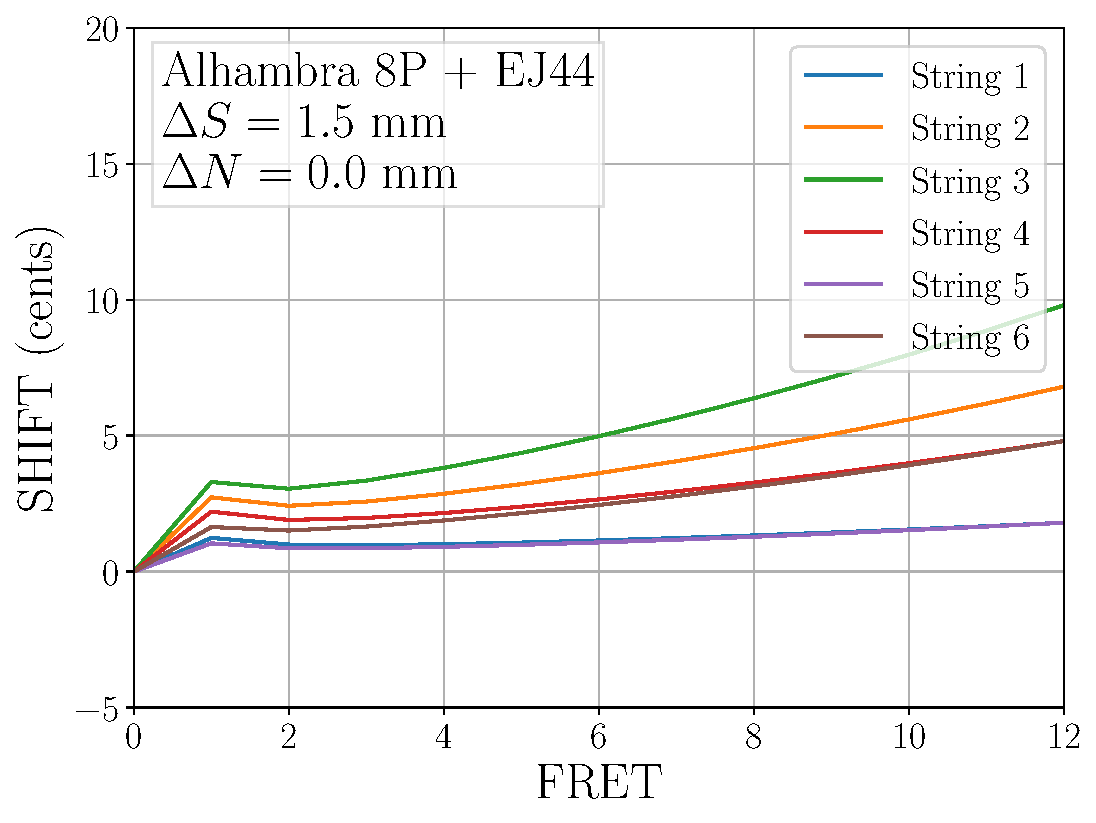
\includegraphics[width=3.25in]{figures/shift_alhambra8p_ej44_factory}
   \caption{Factory guitar}
   \label{fig:shift_alhambra8p_ej44_factory}
  \end{subfigure}
  \par\vspace{0.25in}
  \begin{subfigure}[b]{0.45\textwidth}
   \centering
   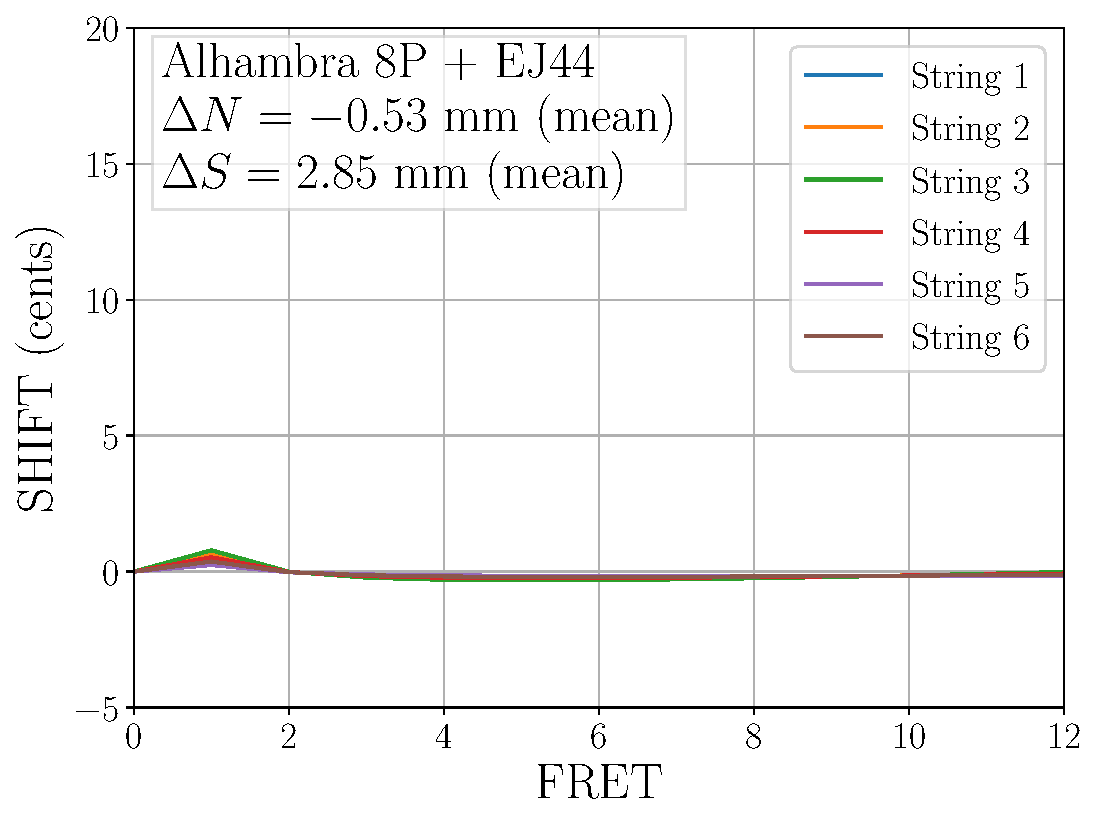
\includegraphics[width=3.25in]{figures/shift_alhambra8p_ej44_full}
   \caption{Full compensation}
   \label{fig:shift_alhambra8p_ej44_full}
  \end{subfigure}
  \hspace{0.25in}
  \begin{subfigure}[b]{0.45\textwidth}
   \centering
   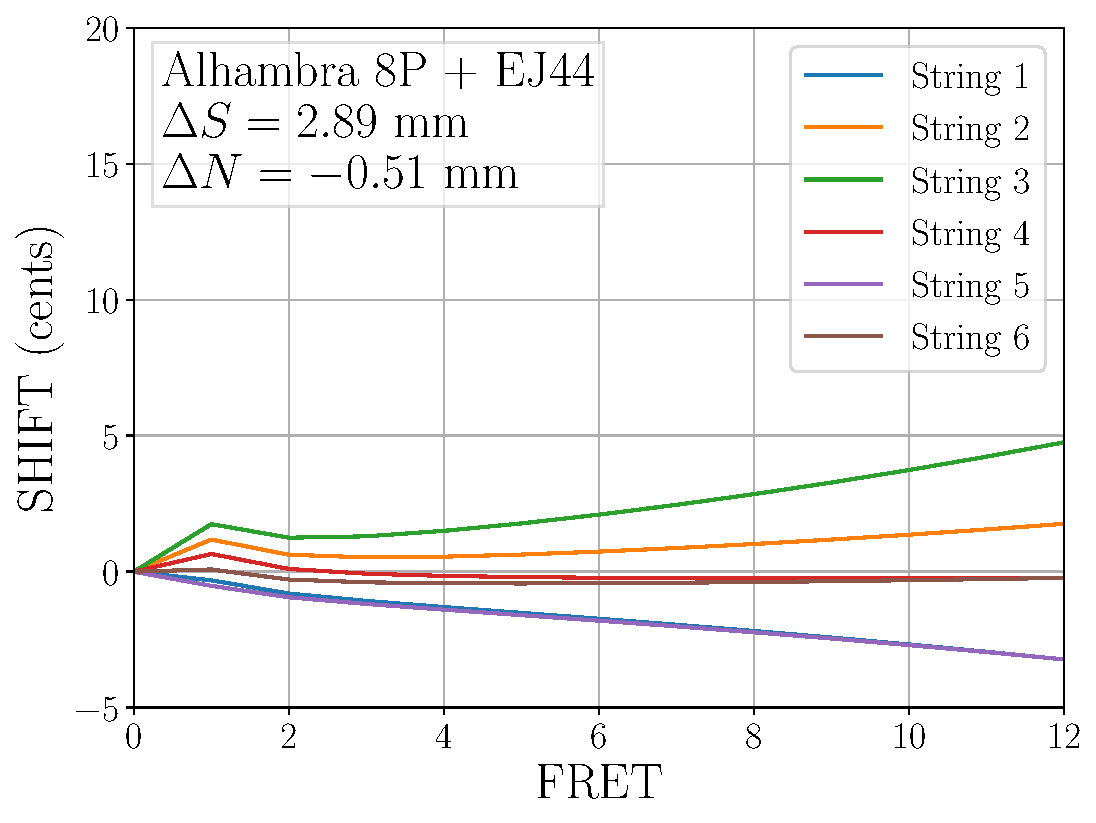
\includegraphics[width=3.25in]{figures/shift_alhambra8p_ej44_mean}
   \caption{Mean compensation}
   \label{fig:shift_alhambra8p_ej44_mean}
  \end{subfigure}
  \caption{\label{fig:compensation_alhambra8p_ej44} Frequency shift (in cents) for an Alhambra 8P guitar with D'Addario Pro-Arte Nylon Classical Guitar Strings -- Extra Hard Tension (EJ44). Four different strategies of saddle and nut compensation are illustrated.}
 \end{figure}
